\chapter{Metodologie}\label{chapter:metodologie}
Questo capitolo esplora il ruolo fondamentale del linguaggio ForgeScript, il linguaggio di scripting del rule engine Forge. Saranno analizzate le caratteristiche distintive del linguaggio di ForgeScript, evidenziandone la flessibilità e la potenza espressiva, e verrà presentato il nuovo linguaggio di scripting Lunar, progettato per migliorare la leggibilità e la gestione degli effetti complessi. Infine, sarà esaminato il processo strategico di addestramento degli LLM, attraverso l'impiego di tecniche avanzate come PEFT \cite{peft} e QLoRA \cite{dettmers2023qlora}, al fine di perfezionare la generazione automatica degli script per le carte in uscita nelle nuove espansioni.


\section{Linguaggio a dominio specifico}\label{sec:dsl}
Un \emph{linguaggio a dominio specifico} (DSL) è un linguaggio di programmazione o di scripting progettato per un ambito particolare di problemi o applicazioni, come nel nostro caso, i giochi di carte collezionabili. A differenza dei linguaggi di programmazione general-purpose, che sono progettati per essere utilizzati in una vasta gamma di contesti, un DSL è ottimizzato per risolvere problemi specifici all'interno di un determinato dominio.

I vantaggi di utilizzare un DSL includono una maggiore espressività, una maggiore facilità di utilizzo da parte degli utenti nel contesto specifico e la possibilità di incorporare concetti e astrazioni rilevanti per il dominio di interesse. Inoltre, i DSL possono semplificare lo sviluppo e la manutenzione del codice, in quanto sono progettati per risolvere problemi specifici e non includono funzionalità superflue \cite{fowler-dsl}.

\section{Extended Backus-Naur Form}\label{sec:ebnf}
EBNF (o \textit{Extended Backus-Naur Form}) è una notazione formale utilizzata per descrivere la sintassi di un linguaggio di programmazione o di un linguaggio di marcatura. È basata sulla forma originale, la Backus-Naur Form (BNF), ma estende le sue capacità per includere una maggiore espressività.

Nella pratica, EBNF viene utilizzata per definire le regole grammaticali di un linguaggio, specificando come le varie parti del linguaggio possono essere combinate per formare espressioni valide. Le regole sono scritte in forma di produzioni, che indicano come combinare i simboli terminali e non terminali per formare costrutti validi nel linguaggio. Ad esempio, una regola EBNF potrebbe definire che un'espressione matematica può essere composta da un numero seguito da un operatore seguito da un altro numero \cite{feynman2016ebnf}.

\section{Il linguaggio di scripting di Forge}\label{sec:forgescript}
Forge utilizza un linguaggio di scripting di nome ForgeScript, ideato dalla community di sviluppatori che contribuiscono al progetto. ForgeScript utilizza una sintassi che descrive le proprietà delle carte attraverso una struttura chiave-valore, la parte più complessa appare nella parte focale della carta, ovvero i suoi effetti, in cui vengono descritte delle variabili (\textbf{SVars} \cite{forge_api}) per identificare gli effetti da chiamare nella livello core del progetto. Il linguaggio non è compilato, ma consiste in un file con estensione \emph{.txt}, che viene letto da un Parser e ne riconosce le funzioni da chiamare all'interno del livello definito \emph{core}. Questo approccio fornisce la possibilità di poter cambiare il comportamento dello scirpt a runtime, dando un vantaggio agli sviluppatori in fase di Debug. ForgeScript  presenta anche delle problematiche per quanto concerne la leggibilità e la gestione degli effetti delle carte più complesse. Considerando la carta in Figura \ref{fig:lightning_helix} per quanto il suo effetto sia tra i più semplici, è un ottimo esempio per capire come il suo equivalente di ForgeScript sia meno intuitivo.

\begin{figure}
	\centering
	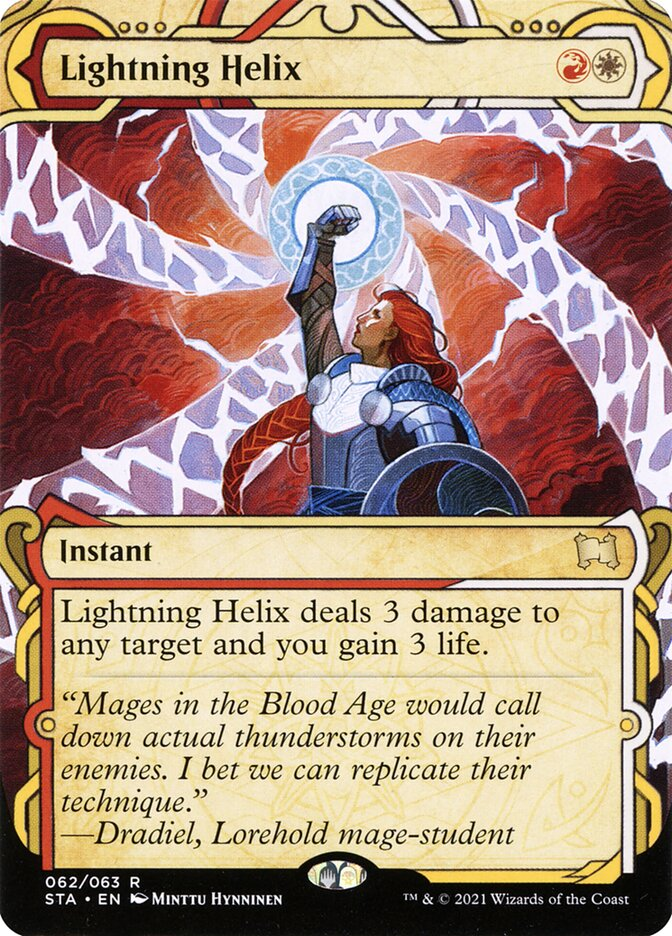
\includegraphics[width=0.6\textwidth]{Immagini/sta-62-lightning-helix.jpg}
	\caption{Carta Lightning Helix con layout Full Art}
	\label{fig:lightning_helix}
\end{figure}


La carta in se permette di infliggere 3 danni ad un qualsiasi bersaglio e di guadagnare 3 punti vita. La risoluzione dei due effetti semplici avviene contemporaneamente, ma prendendo in considerazione lo script descritto dal Codice \ref{lst:lightning_helix_fs}, si può notare come per un effetto semplice si debba creare una variabile che contenga un sotto effetto per guadagnare vita.

\begin{algorithm}
	\caption{Script della carta in Figura \ref{fig:lightning_helix} in ForgeScript}
	\label{lst:lightning_helix_fs}
	\begin{Verbatim}[numbers=left,breaklines]
Name:Lightning Helix
ManaCost:R W
Types:Instant
A:SP$ DealDamage | Cost$ R W | ValidTgts$ Any | NumDmg$ 3 | SubAbility$ DBGainLife | SpellDescription$ CARDNAME deals 3 damage to any target and you gain 3 life.
SVar:DBGainLife:DB$ GainLife | LifeAmount$ 3
Oracle:Lightning Helix deals 3 damage to any target and you gain 3 life.
	\end{Verbatim}
\end{algorithm}


\section{Lunar, un nuovo linguaggio}\label{sec:lunar_dsl}


Lunar nasce dall'idea di sviluppare un nuovo motore di regole per la gestione delle carte nei giochi di carte collezionabili, fornendo il proprio linguaggio di scripting dedicato che abbia come caratteristica principale il fatto di essere facile da imparare, facilmente leggibile per un utente non sviluppatore e che sia facile da adattare alle regole dei singoli GCC. Si ispira alla struttura dei file YAML per rendere l'interazione con il linguaggio più accessibile e intuitiva, riuscendo ad superare le limitazioni analizzate dal linguaggio di scripting di Forge. 

Di seguito, è presentato come potrebbe apparire la struttura di una carta  di \emph{Magic} scritta usando Lunar.

\begin{algorithm}[ht]
	\caption{Struttura di una carta usando Lunar espressa in EBNF}
	\label{lst:ebnf_card}
	\begin{Verbatim}[numbers=left,breaklines]
<card> := <name> <new_line>
          <mana_cost> <new_line>
          <layout> <new_line> 
          <card_type_statement> <new_line> 
          <subtype_statement> <new_line>
          [ <supertype_statement> <new_line> ]
          [ <keywords> ]
          [ <effects> ]
          [ <oracle_text> <new_line> ]
          [ <faces> <new_line> ]
          [ <power> <new_line> ]
          [ <toughness> <new_line> ]
          [ <loyalty> <new_line> ]
          [ <defence> <new_line> ];
	\end{Verbatim}
\end{algorithm}

La sintassi riportata nel Codice \ref{lst:ebnf_card} definisce i diversi elementi che compongono una carta, come il nome, il costo di mana, il tipo di carta, le abilità, gli effetti e così via. Questa struttura fornisce una guida su come scrivere correttamente il codice di una carta usando Lunar, garantendo coerenza e uniformità nella sua definizione.
Questi elementi sono rappresentati come regole grammaticali distinte, ciascuna delle quali è seguita da una nuova riga e da un'indentazione per garantire una maggiore leggibilità.\newline\newline\newline


\begin{algorithm}[!ht]
	\caption{Struttura di effetto di una carta usando Lunar espressa in EBNF}
	\label{lst:ebnf_effect}
    \footnotesize
	\begin{Verbatim} [numbers=left,breaklines]
<effects> := "effects: " <new_line>
                      effect_collection;
<keyword> := "type: " ( "simple" 
                      | "with_amount" 
                      | "with_amount_and_type" 
                      | "with_cost" 
                      | "with_cost_and_type" 
                      | "with_cost_and_amount"
                      | "with_type" ) <new_line>
              "name: " keyword_name new_line
              [ "cost: " {complete_cost}+ <new_line> ]
              [ "amount: " <number> <new_line> ]
              [ "affected_type: " ( <supertype> 
                                  | <card_type> 
                                  | <subtype> ) 
                                 <new_line> ];
         
<effect_collection> :=  {<indent>}+ ( <activated_ability> 
                                    | <triggered_ability>
                                    | <base_ability>
                                    | <complex_ability> ) 
                        <new_line> 
                        {effect_collection};
    \end{Verbatim}
\end{algorithm}

 Di seguito viene riportato il codice scritto in Lunar della carta ``Lightning Helix" raffigurata in Figura \ref{fig:lightning_helix}: come si può notare, il codice scritto in Lunar risulta più chiaro ed è possibile capire che entrambi gli effetti base seguano la stessa gerarchia di risoluzione della versione cartacea.

\begin{algorithm}[!ht]
	\caption{Script della carta in Figura \ref{fig:lightning_helix} in Lunar}
	\label{lst:lightning_helix_ln}
    \footnotesize
	\begin{Verbatim}[numbers=left,breaklines]
name: Lightning Helix
mana_cost: R W
card_type: instant
effects:
    effect:
        type: base
        mode: damage
        target: any_target
        amount: 3
    effect:
        type: base
        mode: life_gain
        target: card_owner
        amount: 3
oracle_text: <Lightning Helix deals 3 damage to any target and you gain 3 life.>
	\end{Verbatim}
\end{algorithm}


Diversamente da ForgeScribe, Lunar offre una sintassi più concisa e con una chiara struttura gerarchica: le proprietà delle carte sono definitae tramite la definizione di coppie chiave-valore. Le abilità e gli effetti possono concatenarsi per ottenere nuove abilità complesse e valide nella grammatica.

Grazie a queste caratteristiche, è possibile rendere Lunar adattabile ai GCC principali, molte delle regole che compongono questi giochi possono essere espressi attraverso le regole di \emph{Magic}. Questo ragionamento può essere facilmente applicabile non solo alle carte da gioco, ma anche alle zone del campo di gioco e alla gestione della struttura del turno.\newline

Di seguito due implementazioni della carta ``Primeval Titan" nei due linguaggi analizzati.


\begin{algorithm}[!ht]
	\caption{Esempio della carta in Figura \ref{fig:one} in ForgeScript}
	\label{lst:prime_titan_fs}
    \footnotesize
	\begin{Verbatim}[numbers=left,breaklines]
Name:Primeval Titan
ManaCost:4 G G
Types:Creature Giant
PT:6/6
K:Trample
T:Mode$ ChangesZone | Origin$ Any | Destination$ Battlefield | ValidCard$ Card.Self | Execute$ TrigChange | OptionalDecider$ You | TriggerDescription$ Whenever CARDNAME enters the battlefield or attacks, you may search your library for up to two land cards, put them onto the battlefield tapped, then shuffle.
T:Mode$ Attacks | ValidCard$ Card.Self | Execute$ TrigChange | TriggerZones$ Battlefield | OptionalDecider$ You | Secondary$ True | TriggerDescription$ Whenever CARDNAME enters the battlefield or attacks, you may search your library for up to two land cards, put them onto the battlefield tapped, then shuffle.
SVar:TrigChange:DB$ ChangeZone | Origin$ Library | Destination$ Battlefield | Tapped$ True | ChangeType$ Land | ChangeNum$ 2 | ShuffleNonMandatory$ True
SVar:HasAttackEffect:TRUE
Oracle:Trample\nWhenever Primeval Titan enters the battlefield or attacks, you may search your library for up to two land cards, put them onto the battlefield tapped, then shuffle. 
	\end{Verbatim}
\end{algorithm}



\begin{algorithm}[!ht]
	\caption{Esempio della carta in Figura \ref{fig:one} in Lunar}
	\label{lst:prime_titan_lunar}
    \footnotesize
	\begin{Verbatim}[numbers=left,breaklines]
name: Primeval Titan
mana_cost: 4 G G
layout: single_face 
card_type: creature
subtype: giant
keywords: 
    keyword:
        type: simple
        name: trample
effects:
    effect:
        type: trigger
        event:
            mode: change_zone
            who: self
            from: anywhere
            to: battlefield
            optional_choice: yes
            optional_decider: card_owner
        event:
            mode: attack
            who: self
            optional_choice: yes
        effect:
            type: base
            mode: move
            from: library
            to: battlefield
            target: land
            amount: 2
            how: tapped
        effect:
            base:
            mode: shuffle
            target: library
oracle_text: <Trample\nWhenever Primeval Titan enters the battlefield or attacks, you may search your library for up to two land cards, put them onto the battlefield tapped, then shuffle.>
power: 6
toughness: 6
	\end{Verbatim}
\end{algorithm}


Sebbene entrambi gli script definiscano la stessa carta, Lunar si distingue per la sua sintassi più pulita e intuitiva, che può rendere il processo di sviluppo e comprensione delle regole del gioco più efficiente e accessibile.
       


\section{PEFT, LoRA e QLoRa}\label{sec:qlora_peft}
Prima di introdurre questi concetti, occorre dare una piccola panoramica su cosa si intende per \textbf{fine-tuning}.
Il fine-tuning nei modelli di linguaggio è un processo cruciale per adattare modelli pre-addestrati alle esigenze specifiche di un compito particolare. Vediamo cosa significa nel contesto degli LLM:

 \begin{enumerate}[label=\alph*.]
    \item  \textbf{Pre-Addestramento}: Gli LLM vengono inizialmente addestrati su grandi quantità di testo non etichettato. Questo processo, chiamato pre-addestramento, consente ai modelli di apprendere rappresentazioni linguistiche generali e di catturare strutture linguistiche complesse.
    
    
    \item  \textbf{Fine-Tuning}: Dopo il pre-addestramento, i modelli possono essere adattati a compiti specifici attraverso il fine-tuning.
        Il fine-tuning coinvolge l’addestramento del modello su un set di dati etichettato specifico per il compito desiderato. Ad esempio, classificazione di testo, traduzione automatica o generazione di testo.
        Durante il fine-tuning, i pesi del modello pre-addestrato vengono aggiornati in base ai nuovi dati etichettati. Tuttavia, solo una piccola parte dei parametri viene addestrata, mantenendo gran parte della conoscenza pre-esistente del modello.

    
    \item  \textbf{Vantaggi del Fine-Tuning}:
        \begin{itemize}
         \item \textit{Efficienza}: Il fine-tuning richiede meno risorse rispetto all’addestramento completo del modello.
         \item \textit{Adattabilità}: Gli LLM pre-addestrati possono essere utilizzati come base per una vasta gamma di compiti senza dover ripartire da zero.
         \item \textit{Prestazioni}: Il fine-tuning consente di ottenere prestazioni competitive su compiti specifici con un investimento computazionale ridotto.
        \end{itemize}  

\end{enumerate}   

    


\subsection{Parameter-Efficient Fine-Tuning}\label{subsec:peft}
PEFT (Parameter-Efficient Fine-Tuning) è un metodo di elaborazione del linguaggio naturale \cite{peft} che offre un modo efficiente per adattare grandi modelli pre-addestrati a diversi compiti specifici senza dover effettuare il fine-tuning di tutti i parametri del modello, il che sarebbe proibitivamente costoso. 

Invece, i metodi PEFT addestrano solo un piccolo numero di parametri aggiuntivi, riducendo significativamente i costi computazionali e di archiviazione, pur ottenendo prestazioni comparabili a un modello al quale è stato applicato un processo di fine-tuning completo.

PEFT offre diversi vantaggi nell’addestramento dei modelli di linguaggio pre-addestrati (PLM):
\begin{enumerate}[label=\alph*.]
    \item   \textbf{Efficienza dei parametri}: PEFT riduce il numero di parametri addestrabili rispetto all’addestramento completo del modello. Questo è particolarmente utile quando si dispone di risorse computazionali limitate o si desidera addestrare rapidamente un modello.
        
    \item  \textbf{Adattatori}: PEFT utilizza adattatori, che sono piccoli strati di rete aggiunti ai blocchi del modello di base. Questi adattatori vengono addestrati separatamente e collegati al modello di base. Ciò consente di adattare il modello a specifici compiti senza dover addestrare l’intero modello da zero.

    \item   \textbf{Riduzione del rischio di overfitting}: Poiché PEFT addestra solo gli adattatori, il rischio di overfitting è ridotto rispetto all’addestramento completo del modello.
    
    \item \textbf{Velocità di addestramento}: PEFT è più veloce dell’addestramento completo del modello, poiché richiede meno iterazioni e meno calcoli.
\end{enumerate}

In sintesi, PEFT offre un modo efficiente per adattare i modelli di linguaggio pre-addestrati a compiti specifici, mantenendo un buon equilibrio tra prestazioni e risorse computazionali.

\subsection{Low-Rank Adaptation}\label{subsec:lora}
LoRA (Low-Rank Adaptation) è una tecnica utilizzata per ridurre la complessità computazionale delle reti neurali durante la distribuzione su dispositivi con risorse limitate, come smartphone, dispositivi per la casa intelligente e sistemi embedded. LoRA consente di adattare modelli pre-addestrati a specifici compiti o domini senza dover ricalcolare tutti i parametri del modello.

LoRA affronta il problema dell'addestramento in due modi fondamentali. Prima di tutto, anziché aggiornare direttamente tutti i  pesi del modello, traccia le modifiche desiderate su tali pesi. Sebbene ciò possa implicare l'aggiunta di ulteriori informazioni da memorizzare, il vantaggio principale risiede nel fatto che le modifiche ai pesi del modello sono tracciate in due matrici separate più piccole. Queste matrici vengono moltiplicate insieme per formare una matrice delle dimensioni del livello della rete neurale al quale si sta applicando il fine-tuning.

Una volta ottenuta questa matrice che rappresenta le modifiche alla traccia iniziale, basterà sommare ciascun elemento di essa alla matrice dei pesi del modello originale.
\begin{figure}[H]
	\centering
	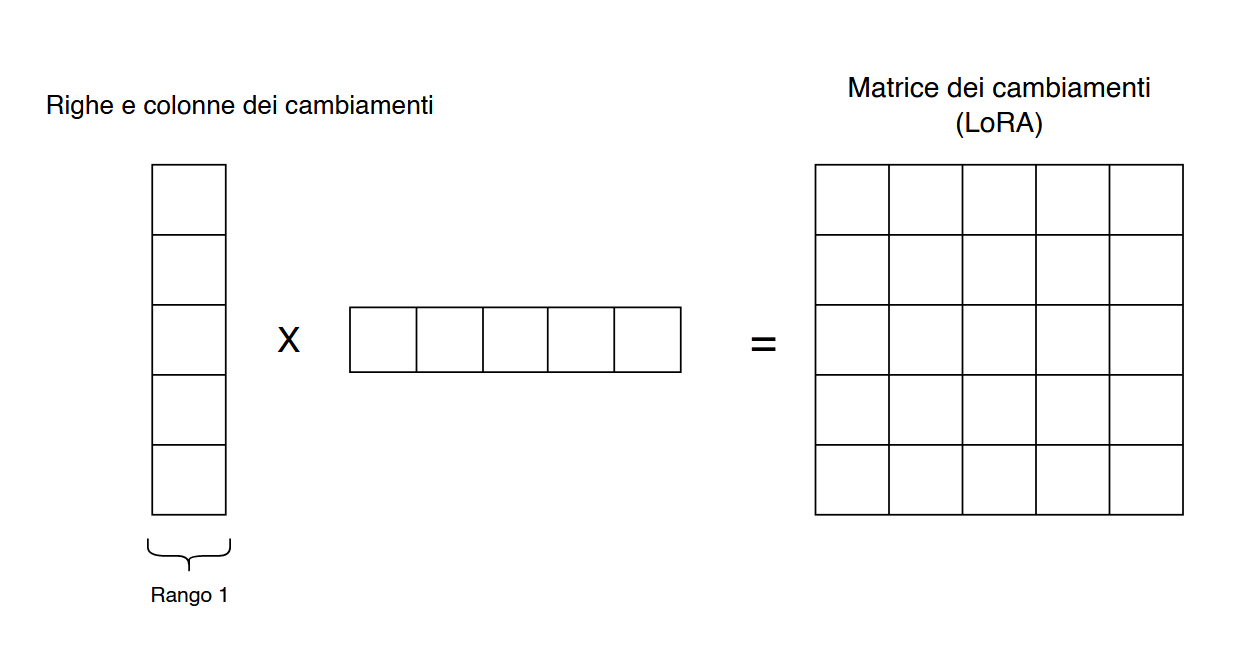
\includegraphics[width=\textwidth]{Immagini/lora_mul.png}
	\caption{Decomposizione di rango}
	\label{fig:lora_mul}
\end{figure}

Soffermandosi nel dettaglio sull'esempio in Figura \ref{fig:lora_mul}, si ottiene la cosiddetta una decomposizione di rango. In questo caso, le matrici di rango 1, contenenti un totale di cinque numeri ciascuna, vengono moltiplicate per formare una matrice di fine-tuning con 25 parametri. Questa strategia sacrifica una certa precisione per un notevole vantaggio in termini di efficienza. 

Dato che si lavora con un numero ridotto di parametri addestrabili, il rango può essere modificato per regolare la precisione dell'output finale. Con un rango più alto si può addestrare una percentuale maggiore dei parametri del modello originale. Tuttavia, poiché i compiti specifici spesso costituiscono solo un sottoinsieme delle capacità del modello, ridurre il rango potrebbe non comportare compromessi significativi in molte situazioni. La capacità di ottenere risultati accurati con aggiornamenti approssimativi, come dimostrato nella ricerca \cite{lora}, è ciò che rende LoRA una soluzione rilevante per questi contesti.

\subsection{Quantized Low-Rank Adaptation}\label{subsec:qlora}
QLoRA (Quantized Low-Rank Adaptation) è un approccio che combina \textbf{quantizzazione} e LoRA.
Nel contesto degli LLM, la quantizzazione si riferisce al processo di conversione dei pesi del modello da tipi di dati a precisione più elevata a quelli a precisione inferiore. In altre parole, i parametri del modello vengono approssimati utilizzando meno bit per rappresentare i loro valori. Questo aiuta a ridurre la memoria richiesta per l’archiviazione dei pesi del modello e a migliorare l’efficienza computazionale durante l’addestramento e l’inferenza. 
Di seguito è presentato il funzionamento (Figura \ref{fig:qlora_v_ft}\footnote{Immagine dal paper QLORA: Efficient Finetuning of Quantized LLMs \cite{dettmers2023qlora}}):

\begin{figure}[H]
	\centering
	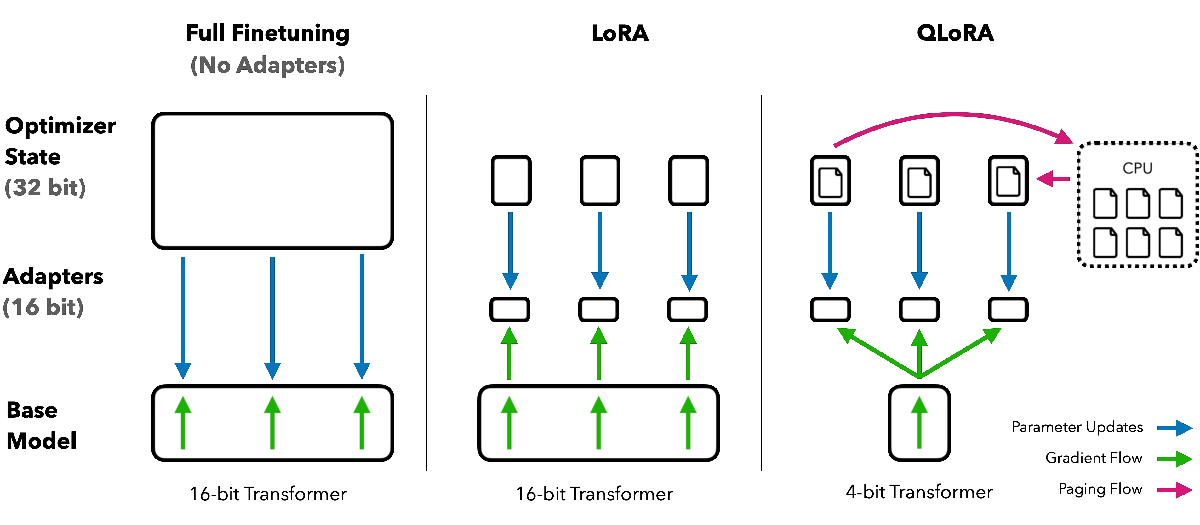
\includegraphics[width=\textwidth]{Immagini/qlora.pdf}
	\caption{Metodi di fine-tuning a confronto}
	\label{fig:qlora_v_ft}
\end{figure}

QLoRA utilizza una tecnica chiamata quantizzazione a 4 bit per comprimere i parametri di un modello linguistico preaddestrato. Questo processo riduce notevolmente lo spazio occupato in memoria senza compromettere le prestazioni del modello.

Una volta che i parametri del modello linguistico sono stati compressi, vengono congelati, il che significa che non vengono più aggiornati durante il fine-tuning. In seguito, vengono aggiunti agli strati del modello un numero limitato di parametri addestrabili (LoRA). Durante il fine-tuning, i gradienti vengono propagati all'indietro attraverso il modello linguistico preaddestrato compresso fino agli Adattatori LoRA, che sono gli unici parametri aggiornati durante l'addestramento.

Un aspetto importante di QLoRA è che utilizza due tipi di dati differenti: un tipo di dato di memorizzazione a 4 bit per i pesi del modello base e un tipo di dato di calcolo a 16 bit per eseguire i calcoli durante il fine-tuning. Questo approccio consente di ridurre l'utilizzo della memoria durante l'addestramento e l'inferenza, poiché i pesi vengono decompressi solo quando sono necessari per eseguire i calcoli.




QLoRA ha portato molti vantaggi nell'addestramento degli LLM, tra cui:

\begin{enumerate}[label=\alph*.]
    \item \textbf{Efficienza}: QLoRA è in grado di elaborare grandi sequenze di dati in modo molto più efficiente rispetto agli LLM tradizionali. Ciò è dovuto al suo meccanismo di attenzione locale basato sulle query, che consente al modello di concentrarsi sulle parti rilevanti dei dati in ingresso.
    
    \item \textbf{Efficacia}: QLoRA può raggiungere un'accuratezza paragonabile a quella degli LLM tradizionali, pur richiedendo risorse computazionali significativamente inferiori. Questo lo rende un'opzione più interessante per gli ambienti con risorse limitate.
    
    \item \textbf{Accessibilità}: L'efficienza di QLoRA lo rende un'opzione più accessibile per i ricercatori e gli sviluppatori che non hanno accesso alle stesse risorse delle grandi istituzioni. Ciò contribuisce a democratizzare l'accesso ai LLM e ad accelerarne l'adozione in diversi settori.
    
    \item \textbf{Prestazioni}: QLoRA è molto efficace nella comprensione e nella generazione del linguaggio naturale. Questo lo rende uno strumento prezioso per le applicazioni che richiedono una profonda comprensione del contesto, come la traduzione linguistica, la creazione di contenuti e persino la risoluzione di problemi complessi.
    
    \item \textbf{Applicazioni in tempo reale:} La capacità di QLoRA di elaborare le informazioni in modo rapido e preciso lo rende ideale per le applicazioni in tempo reale. Ciò è particolarmente significativo in campi come il servizio clienti, dove l'intelligenza artificiale può fornire risposte immediate e contestualmente rilevanti alle richieste degli utenti.


\end{enumerate}

Grazie a QLoRA, è possibile eseguire il fine-tuning di modelli linguistici estremamente grandi su GPU con una quantità limitata di memoria. Inoltre, numerosi esperimenti hanno dimostrato che QLoRA produce risultati comparabili ai metodi tradizionali di fine-tuning a 16 bit, garantendo al contempo una gestione efficiente delle risorse di calcolo e di memoria.

%In sintesi, QLoRA è un'innovazione che democratizza il fine-tuning, consentendo di adattare modelli massicci con miliardi di parametri su GPU relativamente piccole e facilmente disponibili.




